%%%%%%%%%%%%%%%%%%%%%%%%%%%%%%%%%%%%%%%%%%%%%%%%%%%%%%%%%%%%%%%%%%%%%%%%%%%%%%%%
%2345678901234567890123456789012345678901234567890123456789012345678901234567890
%        1         2         3         4         5         6         7         8

\documentclass[letterpaper, 10pt, conference]{ieeeconf}

\IEEEoverridecommandlockouts
\usepackage{cite}
\usepackage{url}
\overrideIEEEmargins
\usepackage{textcomp}
\usepackage{gensymb}
\usepackage{graphicx}
\graphicspath{ {./figures/} }
\usepackage{amsmath}
\usepackage[utf8]{inputenc}
\usepackage{booktabs}

\begin{document}

\title{Experience: Evidence-Aware Pre-Execution Plan Assessment for Generative Robotic Behaviour Planning}

\author{Kalana Ratnayake$^{1}$, Michael Pritchard$^{2}$, Maleen Jayasuriya$^{3}$, Damith Herath$^{4}$%
\thanks{$^{1}$Kalana Ratnayake is with Collaborative Robotics Laboratory, Faculty of Science and Technology, University of Canberra, ACT, Australia {\tt\small Kalana.Ratnayakemudiyanselage@canberra.edu.au}}%
\thanks{$^{2}$Michael Pritchard is with Collaborative Robotics Laboratory, Faculty of Science and Technology, University of Canberra, ACT, Australia {\tt\small Michael.Pritchard@canberra.edu.au}}%
\thanks{$^{3}$Maleen Jayasuriya is with Collaborative Robotics Laboratory, Faculty of Science and Technology, University of Canberra, ACT, Australia {\tt\small Maleen.Jayasuriya@canberra.edu.au}}%
\thanks{$^{4}$Damith Herath is with Collaborative Robotics Laboratory, Faculty of Science and Technology, University of Canberra, ACT, Australia {\tt\small Damith.Herath@canberra.edu.au}}%
}

\maketitle

\begin{abstract}
Generative robotic behaviour planning systems can produce plausible behaviour plans from natural-language tasks, but they still tend to treat generated plans as equally executable until failure occurs at runtime. This is a weak point for deployed robots, because a plan may be semantically relevant while still being slow, fragile, poorly grounded in available behaviour evidence, or mismatched to the robot's state. We introduce \textit{Experience}, a planning layer that sits between behaviour discovery and execution and performs pre-execution plan assessment for generated behaviour execution plans. Experience combines a semantic graph for behaviour and task meaning with a statistical graph for empirical execution evidence, then ranks candidate plans with a Risk-Aware Plan Feasibility Score (RAPFS) that focuses on predicted success, time, energy, fault burden, resource considerations, and epistemic uncertainty. We utilize \textit{Fabric} as a generative behaviour planning system and extend is functionality using the proposed \textit{Experience} stack. We compare the standalone \textit{Fabric} system against the Experience-augmented Fabric system to evaluate the improvements of behaviour plan generation using Experience.
\end{abstract}

\begin{keywords}
robot planning, pre-execution verification, ROS2, risk-aware planning, knowledge graphs, uncertainty-aware ranking
\end{keywords}

\section{Introduction}

Traditional robotic planning systems often rely on pre-defined models and deterministic execution pipelines, which can limit their adaptability and robustness in dynamic environments. These systems typically execute plans under limited variability in real-world conditions, leading to failures when unexpected situations arise. Recently with the popularity of Generative AI, robotics has focused on using LLMs as an potential planning entity to solve these unexpected situations. In \textit{Do as I can, Not as I say} paper \cite{ahn_as_2022} they propose using LLM's semantic knowledge along with robot skills to improve the robot adaptation to dynamic environments. BTGenbot \cite{izzo_btgenbot_2024} focuses on finetuning 7B local LLM model for generating Behaviour Trees while LLM-Brain \cite{lykov_llm-brain_2023} and LLM-BT \cite{zhou_llm-bt_2024}, focus on ... . Fabric is a partially specified FSM \cite{ratnayake2026generativepartiallyspecifiedfinite} that provides capability based generative behaviour planning using graph as a medium.

One of the caveats of these approaches is that they are limited by the context window of the LLM. ... THese generative robotics pipelines can produce plans that read well in language, yet they often forward every available capability description or telemetry fragment into a prompt and defer most feasibility questions until execution time. That pattern is expensive, hard to audit, and unsafe when the robot is operating under resource constraints or partial knowledge.

Recent work has shown that large language models can support long-horizon planning by grounding task descriptions in robot capabilities or scene structure \cite{ahn_as_2022, rana_sayplan_2023}. Behaviour-tree-based systems have pushed this further by generating structured intermediate plans rather than free-form code \cite{izzo_btgenbot_2024, zhou_llm-bt_2024, ao_llm-as-bt-planner_2025}. However, these systems still leave an important gap: candidate plans are rarely ranked using accumulated evidence about how capabilities perform under comparable contexts before execution begins. As a result, the planner may prefer a semantically plausible plan even when the robot has strong prior evidence that the same capability chain is unreliable, too slow, or poorly observed.

Our proposed work augments it with an evidence-aware planning stage. We claim is that pre-execution plan assessment should combine two distinct forms of knowledge: semantic structure, which explains why a behaviour is relevant to the task, and empirical evidence, which estimates how that capability has behaved in comparable contexts. Keeping those roles separate is important because semantic similarity is not equivalent to execution reliability.

We implement the proposed concepts under Experience stack, which is a behaviour-planning extension of Fabric \cite{ratnayake2026generativepartiallyspecifiedfinite}. We utilize Capabilities2 \cite{pritchard_capabilities2_2025} as the behaviour orchestration layer. Experience sits between capability discovery and execution and is intended to consume semantic skill descriptions from Capabilities2 \cite{pritchard_capabilities2_2025, woodall_ros_2014}, observe runtime evidence from the wider ROS 2 system, and improve plan selection before a candidate plan is ranked, selected and dispatched to execution by the Fabric. 

This paper makes three contributions. First, it defines a dual-graph knowledge representation consisting of linked semantic and statistical graphs for behaviour-centric robotic planning. Second, it formulates a Risk-Aware Plan Feasibility Score (RAPFS) that ranks candidate behaviour plans using predicted success, cost, fault burden, and uncertainty. Third, it provides an ROS2 based implementation of the proposed concepts and real world experiment results comparing pre-execution plan assessment against planner outputs that rely primarily on semantic generation alone.

\section{Related Work}

Generative robot planning has moved from direct code generation toward intermediate symbolic structures that can be checked or executed more reliably. SayCan and related systems demonstrated that language-model planning becomes more useful when high-level actions are grounded in embodied capabilities instead of being treated as pure text generation \cite{ahn_as_2022}. SayPlan extended this pattern with scene-graph-based retrieval and iterative refinement for long-horizon tasks \cite{rana_sayplan_2023}. These systems established the value of selective grounding, but they do not by themselves provide a general pre-execution score that compares multiple candidate execution graphs using accumulated runtime evidence.

Behaviour-tree generation systems make the intermediate representation more explicit. BTGenBot, LLM-BT, and LLM-as-BT-Planner show that structured behaviour plans can be generated, validated, and in some cases adapted during execution \cite{izzo_btgenbot_2024, zhou_llm-bt_2024, ao_llm-as-bt-planner_2025}. Their main strength is that the planner output is no longer opaque code. Their main limitation for the present problem is different: a valid plan syntax does not tell us whether the selected plan is the most reliable or feasible one for the current robot state, time budget, or evidence history.

At the capability layer, the original ROS capabilities work and its ROS 2 successor address a different but necessary problem: how robot skills are described, loaded, and composed in a standard way \cite{woodall_ros_2014, pritchard_capabilities2_2025}. Experience builds on that foundation. Capabilities2 provides a structured representation of available robot functionality, but it is not itself a plan-ranking framework. Experience uses those descriptions together with execution evidence to estimate whether a candidate plan is likely to succeed before it is run.

Recent work has been exploring the use of uncertainty measurements to predict whether a task can be achieved or not on the current robotic system. CURE \cite{yin2025reliablellmbasedrobotplanning} proposes a combined uncertainty estimation framework that differentiates between epistemic and intrinsic uncertainty, providing more reliable assessments for LLM-based robot planning. SAFE \cite{guan2025logllmlogbasedanomalydetection} introduces a log-based anomaly detection approach using large language models to enhance the reliability of software systems by identifying potential failures through log analysis. This was rather complex prior to the introduction of LLMs as researchers had to depend of handcrafted rules, regular expressions, and traditional machine learning models for anomaly detection. In Experience, we utilize a similar approach by incorporating ROS2 log collection during runtime to gather evidence about the execution of capabilities, which is then analyzed to predict potential failures and improve the reliability of pre-execution plan assessment.

GraphRAG \cite{edge2025localglobalgraphrag} is used to implement the semantic search and retrieval functionality within a semantic graph, enabling efficient querying and reasoning over the structured knowledge about capabilities, tasks, and context entities. This is mainly focused for Large Document Retrieval tasks, where the system needs to efficiently locate relevant information from a vast collection of documents or knowledge entries. But this approach can be adapted to the robotic planning context, where the semantic graph represents capabilities, tasks, and context entities rather than documents, allowing the system to retrieve relevant knowledge efficiently for plan generation and assessment. EmbodiedRAG \cite{booker2024embodiedragdynamic3dscene} similarly adapts retrieval-augmented generation to dynamic 3D scene graphs for robot task planning, highlighting the potential for RAG-based methods in embodied Robotics contexts.

Experience is an evidence-aware ranking layer placed between generation and execution. This is motivated by a simple observation from the broader fault-tolerance and verification literature: acceptable plans are not defined only by semantic correctness, but also by timing, energy, uncertainty, and the system's ability to justify the choice it made.

\section{Methodology}

\subsection{Problem Formulation}

Let the generative behaviour planner produce a finite candidate set of behaviour-centric execution plans,

\begin{equation}
\mathcal{P}=\{G_{\pi_1}, G_{\pi_2}, \ldots, G_{\pi_m}\},
\end{equation}

where each candidate plan is a directed execution graph,

\begin{equation}
G_{\pi}=(V_{\pi}, E_{\pi}).
\end{equation}

Since we propose the system on capabilities2 \cite{pritchard_capabilities2_2025} framework, each node corresponds to a capability instance or system runner, and each edge represents an execution relationship or triggering condition inherited from the underlying Fabric plan semantics. The research problem is not only to generate these graphs, but to rank them before execution using evidence that is conditioned on the task, context, and prior runtime history.

\subsection{Dual Knowledge Representation}

Experience uses two linked graphs as its knowledge store. The semantic graph in the form of a GraphRAG \cite{edge2025localglobalgraphrag} captures meaning: skill (capability) descriptions, task entities, context entities, reusable plan patterns, and fault concepts. It supports retrieval questions such as which capabilities are relevant to the task, which dependencies frequently co-occur, and which recovery structures are semantically similar to the current problem. The statistical graph contains capabilities as nodes and captures measurement: execution success and failure counts, duration, battery or energy usage, observed fault frequencies, and uncertainty-relevant metadata.

The graphs share stable capability and context identifiers but remain logically separate. This separation prevents a common modeling mistake in generative planning: treating semantic relevance as if it were probability of success. A capability can be a strong semantic match for the user's request and still be a poor operational choice because its empirical evidence is sparse or negative.

\subsection{From Evidence to Node Features}

For each capability instance $i$ in a candidate graph, Experience estimates a feature vector,

\begin{equation}
x_i = [p_i, t_i, e_i, f_i, \mathbf{r}_i, u_i],
\end{equation}

where $p_i$ is estimated success probability, $t_i$ is expected execution time, $e_i$ is expected energy cost, $f_i$ is expected fault burden, $\mathbf{r}_i$ is a resource-demand vector, and $u_i$ is epistemic uncertainty. Epistemic uncertainty combines estimation uncertainty, task ambiguity, unfamiliarity, and missing-evidence penalties which are inspired by the CURE framework \cite{yin2025reliablellmbasedrobotplanning}.

The data for this dual representation is driven by four input classes: runtime observations, capability metadata, prior plan history, and external task context. 

The evaluation resolves candidate plan nodes to stable IDs, retrieves semantic neighbors and statistical data, selects the most specific reliable evidence available, and raises uncertainty when broader fallbacks or missing telemetry are required.

In the current formulation, quantitative resource telemetry is not yet fully available, so the resource vector $\mathbf{r}_i$ remains a declared part of the model while its hard constraint can remain inactive during evaluation.

\subsection{Risk-Aware Plan Feasibility Score}

The Risk-Aware Plan Feasibility Score ranks candidate plans using

\begin{equation}
\operatorname{RAPFS}(G_{\pi}) =
 w_s S(G_{\pi})
 - w_t \hat{T}(G_{\pi})
 - w_e \hat{E}(G_{\pi})
 - w_f \hat{F}(G_{\pi})
 - w_r \hat{C}_r(G_{\pi})
 - w_u \hat{U}(G_{\pi}),
\end{equation}

where $S(G_{\pi})$ is terminal success probability, $\hat{T}(G_{\pi})$, $\hat{E}(G_{\pi})$, $\hat{F}(G_{\pi})$, and $\hat{C}_r(G_{\pi})$ are normalized plan-level costs, and the nonnegative weights encode the deployment trade-off. 

Experience treats failure probability and uncertainty as two distinct concepts. Low success probability indicates that a plan is estimated to fail. High uncertainty indicates that the estimate itself is weak because of sparse evidence, ambiguous task grounding, unfamiliar context, or missing telemetry. Those cases should be handled differently by the planner.

\subsection{Feasibility Constraints and Feedback}

The ranking stage is paired with hard feasibility checks over time, energy, terminal success, and eventually peak concurrent resources and rejects plans that violate   declared limits before execution. During execution, new runtime evidence primarily updates the component-wise statiscal data which will be then used for future plan ranking.

\section{Implementation and Results}

We propose Experience stack as a ROS2 plugin-based framework and an extension for \textit{Fabric} behaviour planning framework \cite{ratnayake2026generativepartiallyspecifiedfinite} which is built on capabilties2 framework. We also propose Supervisor stack as a support mechanism for collecting runtime evidence from the ros2 ecosystem, capabiltiy framework and Fabric framework. It collects execution traces, resource usage, outcome statistics and parses ros2 logs and diagnostics data to feed back into the Experience ranking system.

We also modify the Fabric and capabilities2 frameworks to integrate the Experience system, and to allow Supervisor stack to collect runtime evidence without interfering, ensuring that original functionality is preserved while enabling the collection and utilization of runtime evidence for plan ranking.

The figure \ref{fig:experience_architecture} illustrates the overall architecture of the Experience and Supervisor stacks, showing how runtime evidence is collected and fed back into the plan ranking system.

\begin{figure}
    \centering
    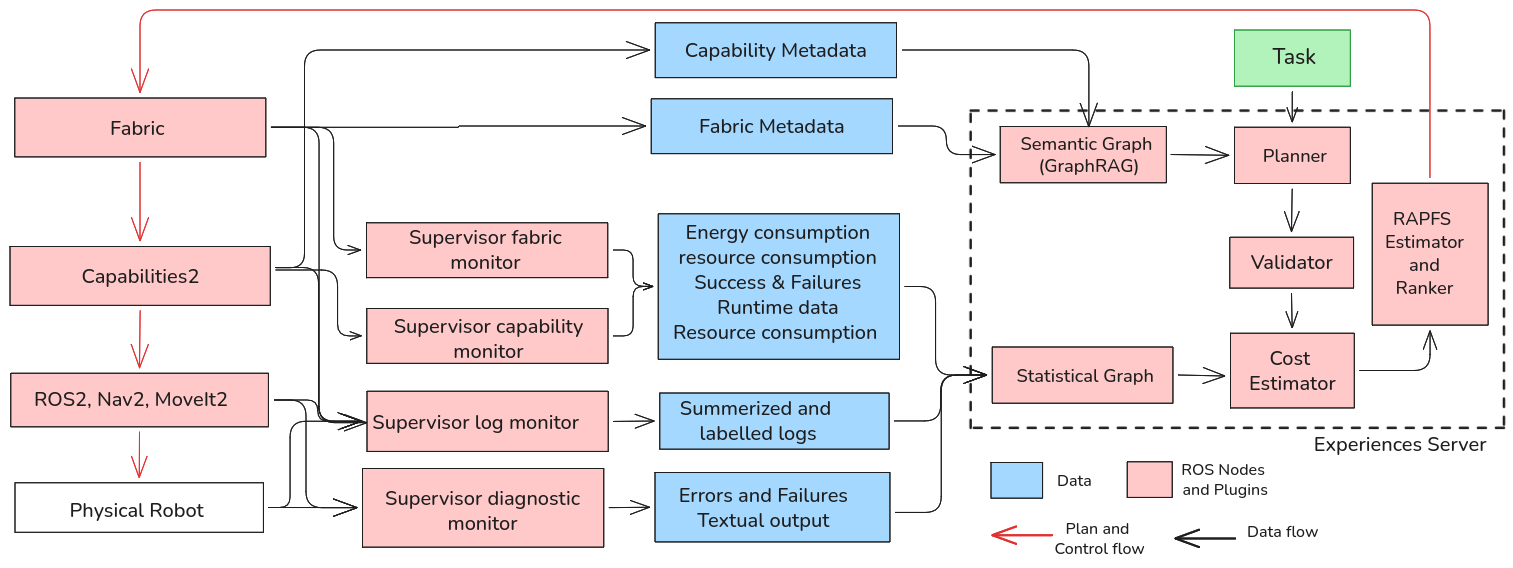
\includegraphics[width=0.8\linewidth]{experience_architecture.png}
    \caption{Architecture of the Experience and Supervisor stacks.}
    \label{fig:experience_architecture}
\end{figure}

We run 5 generative tasks related to manipulation in a Physical Techman TM12s robot as shown in the figure \ref{fig:experiment_setup}. We utilize a custom two finger gripper for the manipulation tasks and a Realsense camera for perception. Anygrasp \cite{fang2023anygrasp} framework is used for grasp pose detection and Ultralytics Yolo26 \cite{jocher2026ultralyticsyolo26unifiedrealtime} is used for object detection. All of these components are integrated into the ROS2 ecosystem to facilitate seamless operation and data collection for the Experience and Supervisor stacks. All the ROS2 nodes run on a local workstation with an Intel Xeon W3245 processor with 192GB RAM and RTX 3090 with 24GB VRAM.

\begin{figure}
    \centering
    \includegraphics[width=0.8\linewidth]{experiment_setup.jpg}
    \caption{Experimental setup with the Physical Techman TM12s robot.}
    \label{fig:experiment_setup}
\end{figure}

The vision and manipulation tasks used for evaluation are as follows:

\begin{enumerate}
    \item Moving the robot to a system level predefined pose. 
    \item Moving the robot through a series of predefined poses.
    \item Counting the number of objects in the scene.
    \item Moving the coke cans in the scene to the drop locations.
    \item Moving one of the oranges to the drop location.
\end{enumerate}

These tasks are evaluated under 3 conditions and each task is iterated 10 times. Following are the evaluation conditions:

\begin{enumerate}
    \item Fabric stack for direct plan generation.
    \item Fabric and Experience stacks with Experience containing only semantic information.
    \item Fabric and Experience stacks with Experience containing both semantic information and empirical run evidence.
\end{enumerate}

In the second evaluation condition, the Experience stack contains only semantic information, and expects the experience stack to gain empirical run evidence over time as tasks are executed. In the third evaluation condition, the Experience stack already contains empirical run evidence collected from non-generative predefined plan executions. It is also expected to collect run evidence during the evaluation, allowing the system to leverage both prior experience and empirical run evidence for more informed plan selection.

\section{Conclusion}

Experience is intended to make generative robot planning more selective and more defensible before execution begins. It emphasizes that plan candidates should not be ranked only by how well they match the task in language, but also by how well prior evidence suggests they will execute under the current conditions. The dual-graph representation and RAPFS formulation provide that bridge between semantic relevance and empirical feasibility.

This initial paper draft captures the contribution's conceptual center from the canonical Contribution 2 markdown source. What remains unfinished is primarily empirical packaging, not the architectural argument. The next stage is to consolidate the evaluation evidence into a paper-specific results section that tests whether Experience improves plan ranking, calibration, and failure avoidance relative to generation-only baselines.

\bibliographystyle{ieeetr}
\bibliography{references}

\end{document}
